\documentclass[tikz]{standalone}
\usetikzlibrary{shapes.geometric}
\begin{document}%
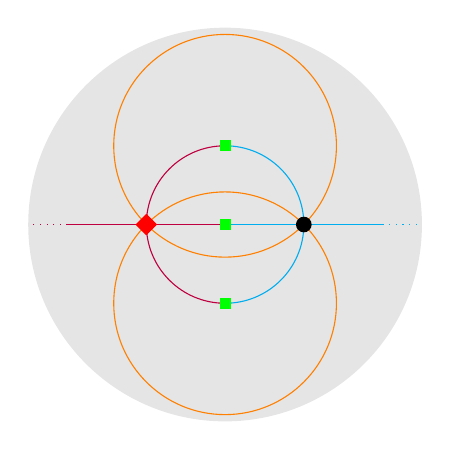
\begin{tikzpicture}
\fill[gray!20] (0,0) circle (2.5cm);

\coordinate (A) at (1,0);
\coordinate (C) at (-1,0);
\coordinate (B0) at (0,1);
\coordinate (B1) at (0,0);
\coordinate (B2) at (0,-1);

\draw[purple] (C) -- (B1);
\draw[purple] (C) -- (-2,0);
\draw[purple,dotted] (-2,0) -- (-2.5,0);
\draw[purple] (0,-1) arc [start angle=270, end angle=180, radius=1];
\draw[purple] (0,1) arc [start angle=90, end angle=180, radius=1];

\draw[cyan] (A) -- (B1);
\draw[cyan] (A) -- (2,0);
\draw[cyan,dotted] (2,0) -- (2.5,0);
\draw[cyan] (0,-1) arc [start angle=270, end angle=360, radius=1];
\draw[cyan] (0,1) arc [start angle=90, end angle=0, radius=1];

\draw[orange] (0,1) circle [radius=1.4142];
\draw[orange] (0,-1) circle [radius=1.4142];

\node[diamond,fill=red,inner sep=2pt] at (C) {};
\node[circle,fill=black,inner sep=2pt] at (A) {};
\foreach \x in {0,1,2}
\node[rectangle,fill=green,inner sep=2pt] at (B\x) {};

\end{tikzpicture}%
\end{document}
